% Options for packages loaded elsewhere
% Options for packages loaded elsewhere
\PassOptionsToPackage{unicode}{hyperref}
\PassOptionsToPackage{hyphens}{url}
\PassOptionsToPackage{dvipsnames,svgnames,x11names}{xcolor}
%
\documentclass[
  number,
  preprint]{elsarticle}
\usepackage{xcolor}
\usepackage[margin=0.55in]{geometry}
\usepackage{amsmath,amssymb}
\setcounter{secnumdepth}{5}
\usepackage{iftex}
\ifPDFTeX
  \usepackage[T1]{fontenc}
  \usepackage[utf8]{inputenc}
  \usepackage{textcomp} % provide euro and other symbols
\else % if luatex or xetex
  \usepackage{unicode-math} % this also loads fontspec
  \defaultfontfeatures{Scale=MatchLowercase}
  \defaultfontfeatures[\rmfamily]{Ligatures=TeX,Scale=1}
\fi
\usepackage{lmodern}
\ifPDFTeX\else
  % xetex/luatex font selection
\fi
% Use upquote if available, for straight quotes in verbatim environments
\IfFileExists{upquote.sty}{\usepackage{upquote}}{}
\IfFileExists{microtype.sty}{% use microtype if available
  \usepackage[]{microtype}
  \UseMicrotypeSet[protrusion]{basicmath} % disable protrusion for tt fonts
}{}
\makeatletter
\@ifundefined{KOMAClassName}{% if non-KOMA class
  \IfFileExists{parskip.sty}{%
    \usepackage{parskip}
  }{% else
    \setlength{\parindent}{0pt}
    \setlength{\parskip}{6pt plus 2pt minus 1pt}}
}{% if KOMA class
  \KOMAoptions{parskip=half}}
\makeatother
% Make \paragraph and \subparagraph free-standing
\makeatletter
\ifx\paragraph\undefined\else
  \let\oldparagraph\paragraph
  \renewcommand{\paragraph}{
    \@ifstar
      \xxxParagraphStar
      \xxxParagraphNoStar
  }
  \newcommand{\xxxParagraphStar}[1]{\oldparagraph*{#1}\mbox{}}
  \newcommand{\xxxParagraphNoStar}[1]{\oldparagraph{#1}\mbox{}}
\fi
\ifx\subparagraph\undefined\else
  \let\oldsubparagraph\subparagraph
  \renewcommand{\subparagraph}{
    \@ifstar
      \xxxSubParagraphStar
      \xxxSubParagraphNoStar
  }
  \newcommand{\xxxSubParagraphStar}[1]{\oldsubparagraph*{#1}\mbox{}}
  \newcommand{\xxxSubParagraphNoStar}[1]{\oldsubparagraph{#1}\mbox{}}
\fi
\makeatother

\usepackage{color}
\usepackage{fancyvrb}
\newcommand{\VerbBar}{|}
\newcommand{\VERB}{\Verb[commandchars=\\\{\}]}
\DefineVerbatimEnvironment{Highlighting}{Verbatim}{commandchars=\\\{\}}
% Add ',fontsize=\small' for more characters per line
\usepackage{framed}
\definecolor{shadecolor}{RGB}{241,243,245}
\newenvironment{Shaded}{\begin{snugshade}}{\end{snugshade}}
\newcommand{\AlertTok}[1]{\textcolor[rgb]{0.68,0.00,0.00}{#1}}
\newcommand{\AnnotationTok}[1]{\textcolor[rgb]{0.37,0.37,0.37}{#1}}
\newcommand{\AttributeTok}[1]{\textcolor[rgb]{0.40,0.45,0.13}{#1}}
\newcommand{\BaseNTok}[1]{\textcolor[rgb]{0.68,0.00,0.00}{#1}}
\newcommand{\BuiltInTok}[1]{\textcolor[rgb]{0.00,0.23,0.31}{#1}}
\newcommand{\CharTok}[1]{\textcolor[rgb]{0.13,0.47,0.30}{#1}}
\newcommand{\CommentTok}[1]{\textcolor[rgb]{0.37,0.37,0.37}{#1}}
\newcommand{\CommentVarTok}[1]{\textcolor[rgb]{0.37,0.37,0.37}{\textit{#1}}}
\newcommand{\ConstantTok}[1]{\textcolor[rgb]{0.56,0.35,0.01}{#1}}
\newcommand{\ControlFlowTok}[1]{\textcolor[rgb]{0.00,0.23,0.31}{\textbf{#1}}}
\newcommand{\DataTypeTok}[1]{\textcolor[rgb]{0.68,0.00,0.00}{#1}}
\newcommand{\DecValTok}[1]{\textcolor[rgb]{0.68,0.00,0.00}{#1}}
\newcommand{\DocumentationTok}[1]{\textcolor[rgb]{0.37,0.37,0.37}{\textit{#1}}}
\newcommand{\ErrorTok}[1]{\textcolor[rgb]{0.68,0.00,0.00}{#1}}
\newcommand{\ExtensionTok}[1]{\textcolor[rgb]{0.00,0.23,0.31}{#1}}
\newcommand{\FloatTok}[1]{\textcolor[rgb]{0.68,0.00,0.00}{#1}}
\newcommand{\FunctionTok}[1]{\textcolor[rgb]{0.28,0.35,0.67}{#1}}
\newcommand{\ImportTok}[1]{\textcolor[rgb]{0.00,0.46,0.62}{#1}}
\newcommand{\InformationTok}[1]{\textcolor[rgb]{0.37,0.37,0.37}{#1}}
\newcommand{\KeywordTok}[1]{\textcolor[rgb]{0.00,0.23,0.31}{\textbf{#1}}}
\newcommand{\NormalTok}[1]{\textcolor[rgb]{0.00,0.23,0.31}{#1}}
\newcommand{\OperatorTok}[1]{\textcolor[rgb]{0.37,0.37,0.37}{#1}}
\newcommand{\OtherTok}[1]{\textcolor[rgb]{0.00,0.23,0.31}{#1}}
\newcommand{\PreprocessorTok}[1]{\textcolor[rgb]{0.68,0.00,0.00}{#1}}
\newcommand{\RegionMarkerTok}[1]{\textcolor[rgb]{0.00,0.23,0.31}{#1}}
\newcommand{\SpecialCharTok}[1]{\textcolor[rgb]{0.37,0.37,0.37}{#1}}
\newcommand{\SpecialStringTok}[1]{\textcolor[rgb]{0.13,0.47,0.30}{#1}}
\newcommand{\StringTok}[1]{\textcolor[rgb]{0.13,0.47,0.30}{#1}}
\newcommand{\VariableTok}[1]{\textcolor[rgb]{0.07,0.07,0.07}{#1}}
\newcommand{\VerbatimStringTok}[1]{\textcolor[rgb]{0.13,0.47,0.30}{#1}}
\newcommand{\WarningTok}[1]{\textcolor[rgb]{0.37,0.37,0.37}{\textit{#1}}}

\usepackage{longtable,booktabs,array}
\newcounter{none} % for unnumbered tables
\usepackage{calc} % for calculating minipage widths
% Correct order of tables after \paragraph or \subparagraph
\usepackage{etoolbox}
\makeatletter
\patchcmd\longtable{\par}{\if@noskipsec\mbox{}\fi\par}{}{}
\makeatother
% Allow footnotes in longtable head/foot
\IfFileExists{footnotehyper.sty}{\usepackage{footnotehyper}}{\usepackage{footnote}}
\makesavenoteenv{longtable}
\usepackage{graphicx}
\makeatletter
\newsavebox\pandoc@box
\newcommand*\pandocbounded[1]{% scales image to fit in text height/width
  \sbox\pandoc@box{#1}%
  \Gscale@div\@tempa{\textheight}{\dimexpr\ht\pandoc@box+\dp\pandoc@box\relax}%
  \Gscale@div\@tempb{\linewidth}{\wd\pandoc@box}%
  \ifdim\@tempb\p@<\@tempa\p@\let\@tempa\@tempb\fi% select the smaller of both
  \ifdim\@tempa\p@<\p@\scalebox{\@tempa}{\usebox\pandoc@box}%
  \else\usebox{\pandoc@box}%
  \fi%
}
% Set default figure placement to htbp
\def\fps@figure{htbp}
\makeatother





\setlength{\emergencystretch}{3em} % prevent overfull lines

\providecommand{\tightlist}{%
  \setlength{\itemsep}{0pt}\setlength{\parskip}{0pt}}



 
\usepackage[]{natbib}
\bibliographystyle{elsarticle-num}


\usepackage{tikz}
\usetikzlibrary{shapes.geometric, arrows.meta, positioning, fit, backgrounds}
\makeatletter
\@ifpackageloaded{caption}{}{\usepackage{caption}}
\AtBeginDocument{%
\ifdefined\contentsname
  \renewcommand*\contentsname{Table of contents}
\else
  \newcommand\contentsname{Table of contents}
\fi
\ifdefined\listfigurename
  \renewcommand*\listfigurename{List of Figures}
\else
  \newcommand\listfigurename{List of Figures}
\fi
\ifdefined\listtablename
  \renewcommand*\listtablename{List of Tables}
\else
  \newcommand\listtablename{List of Tables}
\fi
\ifdefined\figurename
  \renewcommand*\figurename{Figure}
\else
  \newcommand\figurename{Figure}
\fi
\ifdefined\tablename
  \renewcommand*\tablename{Table}
\else
  \newcommand\tablename{Table}
\fi
}
\@ifpackageloaded{float}{}{\usepackage{float}}
\floatstyle{ruled}
\@ifundefined{c@chapter}{\newfloat{codelisting}{h}{lop}}{\newfloat{codelisting}{h}{lop}[chapter]}
\floatname{codelisting}{Listing}
\newcommand*\listoflistings{\listof{codelisting}{List of Listings}}
\makeatother
\makeatletter
\makeatother
\makeatletter
\@ifpackageloaded{caption}{}{\usepackage{caption}}
\@ifpackageloaded{subcaption}{}{\usepackage{subcaption}}
\makeatother
\journal{Template Journal}
\usepackage{bookmark}
\IfFileExists{xurl.sty}{\usepackage{xurl}}{} % add URL line breaks if available
\urlstyle{same}
\hypersetup{
  pdftitle={GNC Assignment: Solution Approach},
  pdfauthor={Kiran M Aralikatti},
  colorlinks=true,
  linkcolor={blue},
  filecolor={Maroon},
  citecolor={Blue},
  urlcolor={Blue},
  pdfcreator={LaTeX via pandoc}}


\setlength{\parindent}{6pt}
\begin{document}

\begin{frontmatter}
\title{GNC Assignment: Solution Approach \\\large{Bellatrix Aerospace
Pvt. Ltd} }
\author[]{Kiran M Aralikatti%
%
}





        





\end{frontmatter}
    

\section{Introduction}\label{sec-introduction}

The document contains the various solution methods for the GNC
assignment problems. The given problems can be solved using more then
one method, which author tried to implement. The document generated
using \href{https://quarto.org/docs/journals/}{Quarto} locally, created
by the author. The source remains editable as a normal \texttt{.qmd}
manuscript and the template can be found
\href{https://github.com/kirancoder/paper_template/tree/main/sample_paper}{here}.

\section{Task 1}\label{sec-task1}

This is a very intersting geometery problem, which can solved using
trignometric relations to a triangles in a minor sector and also
converting the problem in polar co-ordinates.

The 1st and formost the cone has to opened and converted into a sector
of a circle, for a given right circular cone in the problem, it will
always be a minor sector of a circle. For both the methods, minor sector
will be used to find the downhill distance.

The 2nd catch is, when the cone is opened, the curve connecting point A
and B will be stright line, which is the shortest distance between two
points.

The below image shows the above discussed points, where the cone is
opened and the curve connecting A and B is stright line.

\begin{figure}[H]

\begin{minipage}[t]{0.50\linewidth}

\centering{

\pandocbounded{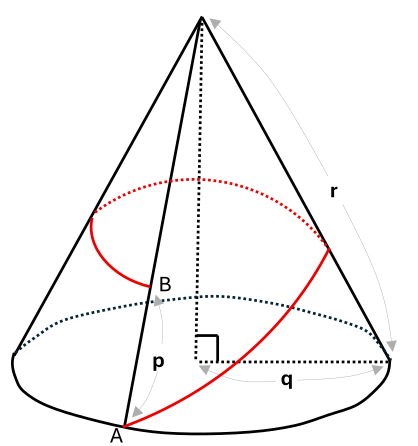
\includegraphics[keepaspectratio]{images/GNC_img_1.png}}

}

\subcaption{\label{fig-given-cone}}

\end{minipage}%
%
\begin{minipage}[t]{0.50\linewidth}

\centering{

\pandocbounded{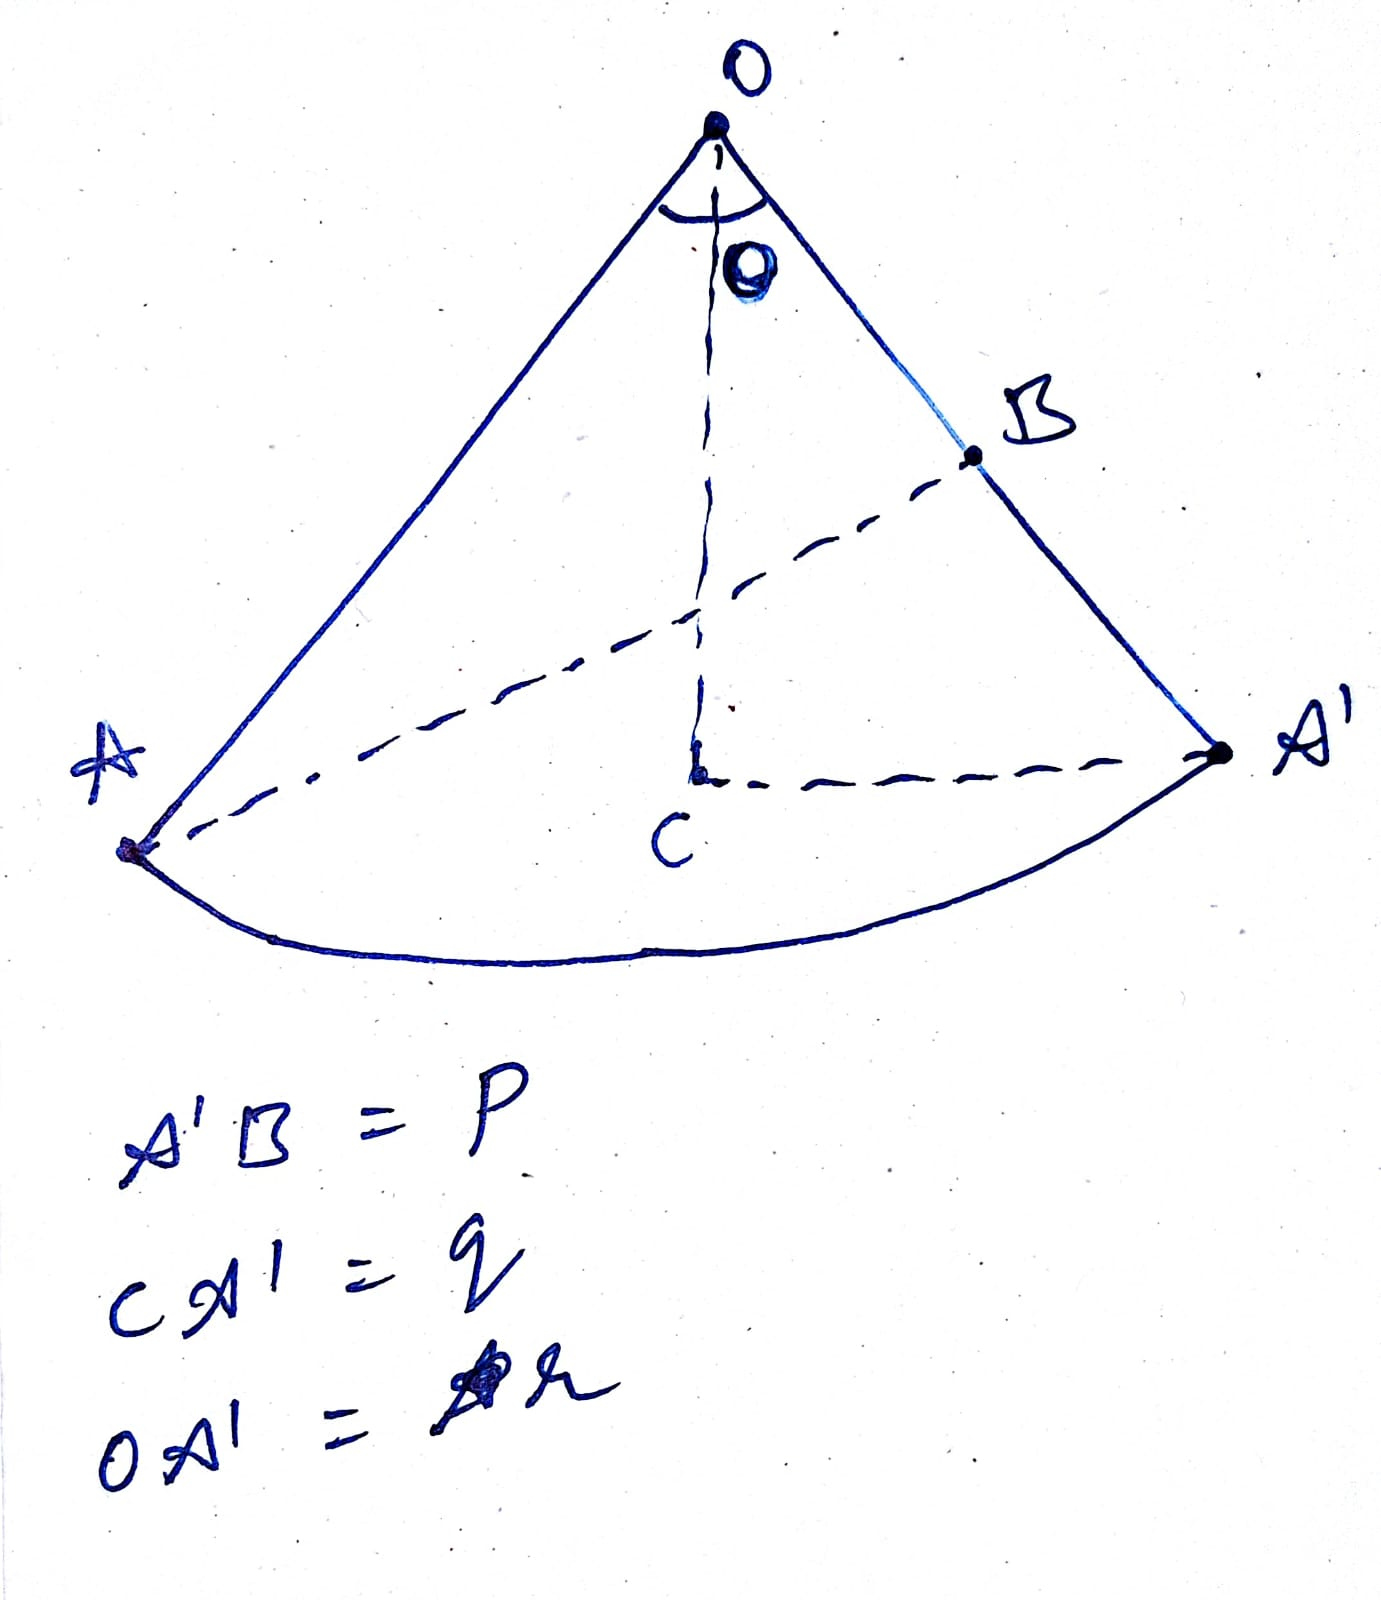
\includegraphics[keepaspectratio]{images/GNC_img_2.png}}

}

\subcaption{\label{fig-opened-cone}}

\end{minipage}%

\caption{\label{fig-cone}Given cone and its corresponding sector
representation.}

\end{figure}%

\subsection{Solution 1}\label{sec-task1-sol1}

In the given Figure~\ref{fig-opened-cone}, shows that the lengths of the
given cone ``p, q, r'' relation to the various lenths of the minor
sector.

Considering the person is going from the point A to B, the downhill
distance will lie on the somewhere on the line connecting A and B. The
distance can be calculated using trignometric relations to the triangle
\(\Delta \;ABO\) formed in the minor sector \(OAA'\).

To define the uphill while moving on the line AB, one can imgaine moving
closer to the point O, i.e.~and then moving away from the point O, until
reaching the point B. The divide the line segement AB into two parts,
uphill and downhill, we a need a point of AB, which lies close to the
point O, this can be found by draiwing a perpendicular from the point O
to the line AB, which will intersect at a point D. The point D will be
the closest point to O on the line AB, and hence the point D will be the
point where the uphill ends and downhill starts.

The below image will show the point D in the \(\Delta \;ABO\) triangle,
which is the closest point to O on the line AB.

\begin{figure}[H]

\begin{minipage}[t]{\linewidth}

\pandocbounded{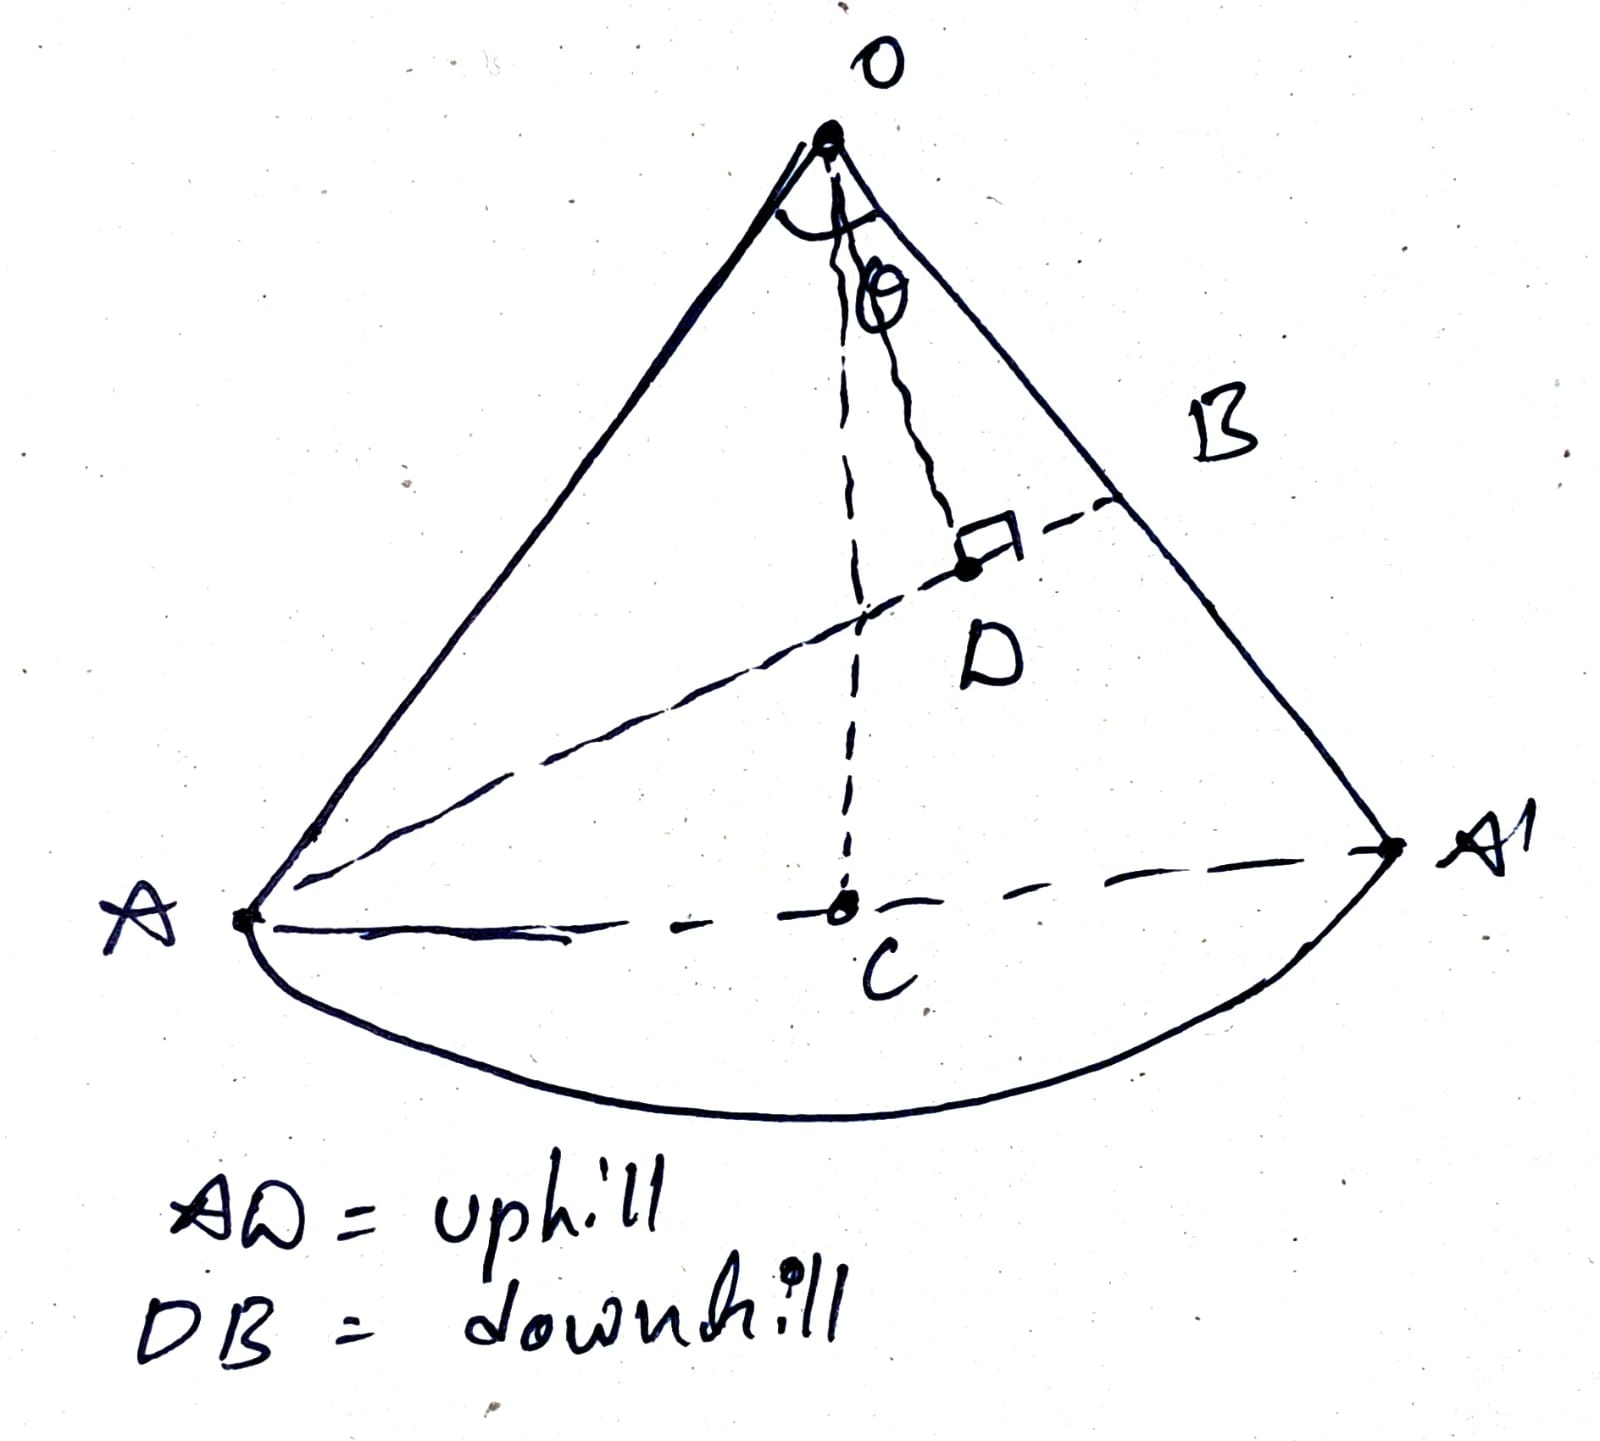
\includegraphics[keepaspectratio]{images/GNC_img_3.png}}

\end{minipage}%

\caption{\label{fig-cone}Representation of the uphill and downhill
paths.}

\end{figure}%

So the task is now to find the distance DB, as the function of the given
lengths p, q and r.

The \(\Delta \; ABO\) the \(\angle\; \theta\), is common between the
\(\Delta \; ABO\) and the sector. By the realtion between the angle and
arc in circle,
\begin{equation}\protect\phantomsection\label{eq-r_theta}{
\theta = \frac{l}{r}
}\end{equation}

where \(l = \overset{\frown}{AB}\) and \(r\) is radius and \(\theta\) is
angle suspended by the sector.

The lengths \(q\) which is the radius of the cone, the permeter of the
sector can derivied from that,
\begin{equation}\protect\phantomsection\label{eq-cone}{
\overset{\frown}{AB} = 2\, \pi \, q
}\end{equation}

Now, substiting arc length relation into Equation~\ref{eq-r_theta},

\[
\theta = \frac{2\, \pi \, q}{r}
\]

Hence, \(\theta  = f(q,r)\).

Now, in \(\Delta AOB\), and \(\theta\) and two sides (\(OA = r\) \&
\(OB = r - p\)) known in terms of the known quantites, so we can now
apply \(cosine\) rule to find the third side, \(AB\) in terms of given
parameters \(p, \; q \& r\)

\begin{equation}\protect\phantomsection\label{eq-cosine}{
{AB}^2 = {OA}^2 + {OB}^2 - 2 \cdot OA \cdot OB \; cos(\theta) = r^2+(r-p)^2-2r(r-p)\cos\theta
}\end{equation}

Consider \(AB = k\)

\[
k = \sqrt{r^2+(r-p)^2-2r(r-p)\cos\theta}
\]

Now, for the \(\Delta AOD\) and \(\Delta DOB\) are right angle
triangles, the side \(OD\):
\begin{equation}\protect\phantomsection\label{eq-tri-rel}{
\begin{aligned}
OD^2 = OA^2 - AD^2 \quad \text{in } \Delta AOD \\
OD^2 = OB^2 - BD^2 \quad \text{in } \Delta DOB
\end{aligned}
}\end{equation}

For simiplification consider \(AD = m \; \text{and} \; DB = n\) which is
line \(AB\) defined above, then from Equation~\ref{eq-tri-rel} \[
r^2 - m^2 = (r-p)^2 - n^2
\]

here \(m\) is uphill distance and \(n\) is downhill distance and
simplifying the above solution gives,
\begin{equation}\protect\phantomsection\label{eq-main}{
\begin{aligned}
m^2 - n^2 = r^2 - (r-p)^2 \\
(m+n)(m-n) = r^2 - (r-p)^2
\end{aligned}
}\end{equation}

then,

\begin{equation}\protect\phantomsection\label{eq-main-2}{
m-n = \frac{r^2 - (r-p)^2}{m+n} = \frac{r^2 - (r-p)^2}{k} 
}\end{equation}

and from the relations of \(k, m \; \text{and} \; n\),
\begin{equation}\protect\phantomsection\label{eq-main-1}{
m + n = k
}\end{equation}

Now, substract Equation~\ref{eq-main-2} from Equation~\ref{eq-main-1}
gives

\[
\begin{aligned}
2n = \frac{k^2 - r^2 + (r-p)^2}{k}
\end{aligned}
\]

Substitute the value of \(k\) and simplify,

\[
\begin{aligned}
n = \frac{(r-p)^2 - r(r-p) cos(\theta)}{\sqrt{r^2+(r-p)^2-2r(r-p)\cos\theta}}
\end{aligned}
\]

So, the downhill distance (\(n\)), is the function
\(p, q, \text{and} r\) as \(\theta\) is also function of
\(p, q, \; \text{and} \; r\)

\[
n = g(p, q, r)
\]

This can also be solved using polar co-oridnates
(\(r \; \text{and} \; \theta\)) and minimum distance and other required
relations formed in that form.

\pagebreak

\section{Task 2}\label{sec-task2}

This task is about the parameters estimation of the spring-mass-damper
system, for the given mass and velocity data. This can be posed as a
optimization problem, such that design varibles are damping and spring
coefficients and the obejective function as \(\Delta V\), i.e.~the
difference between simulation and given data, with the constraints as
\(2^{nd}\) order dynamics of the system.

\subsection{Solution Method}\label{solution-method}

As per the problem statement, the same spring is used i.e.~which expands
the same length which is \(0.15 \; m\) every time.

Let's consider the states of the system, position and velocity at
\(t_0\), which are \([-0.15, 0.0]\). The positon is initially taken as
negative, because at final time the body is experiences only zero spring
force \(F(t_f) = kx =0\), as \(k\) can't be zero, we conclude that
\(x(t_f)=0\).

The final states are, \([0.0, v_{data}]\).

\begin{equation}\protect\phantomsection\label{eq-x1}{
\dot{x}_1 = x_2
}\end{equation}

\begin{equation}\protect\phantomsection\label{eq-x2}{
\dot{x}_2 = -\frac{b}{m}x_2 - \frac{k}{m}x_1
}\end{equation}

Initial Conditions:

\begin{equation}\protect\phantomsection\label{eq-bc-x1}{
x_1(t_0) = -0.15
}\end{equation}

\begin{equation}\protect\phantomsection\label{eq-bc-x2}{
x_2(t_0) = 0.0
}\end{equation}

Final Conditions:

\begin{equation}\protect\phantomsection\label{eq-bc1-x1}{
x_1(t_f) = 0.0
}\end{equation}

\begin{equation}\protect\phantomsection\label{eq-bc1-x2}{
x_2(t_f) = \mathrm{data}
}\end{equation}

\begin{center}
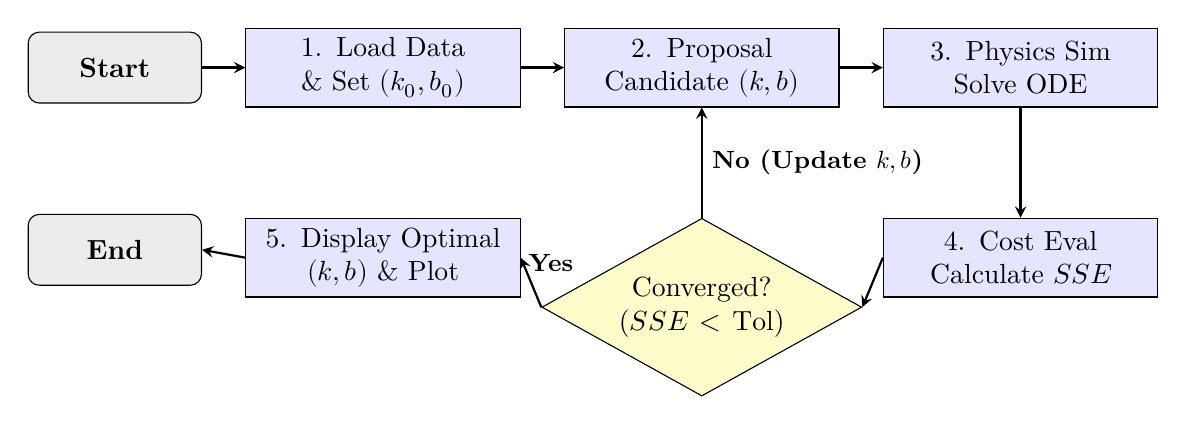
\begin{tikzpicture}[
    node distance=1.2cm and 0.55cm,
    scale=1.0,
    transform shape,
    startstop/.style={
        rectangle,
        rounded corners,
        minimum width=2.2cm,
        minimum height=0.9cm,
        text centered,
        draw=black,
        fill=gray!15,
        font=\bfseries
    },
    process/.style={
        rectangle,
        minimum width=3.25cm,
        minimum height=1.0cm,
        text centered,
        text width=3.25cm,
        draw=black,
        fill=blue!10
    },
    decision/.style={
        diamond,
        aspect=1.8,
        minimum width=2.7cm,
        minimum height=1.1cm,
        text centered,
        text width=2.7cm,
        draw=black,
        fill=yellow!20,
        inner sep=0pt
    },
    arrow/.style={
        thick,
        ->,
        >=stealth
    }
]
% TOP ROW
\node (start) [startstop] {Start};
\node (init) [process, right=of start] {1. Load Data \\ \& Set $(k_0,b_0)$};
\node (opt) [process, right=of init] {2. Proposal \\ Candidate $(k,b)$};
\node (sim) [process, right=of opt] {3. Physics Sim \\ Solve ODE};
% BOTTOM ROW
\node (cost) [process, below=1.4cm of sim] {4. Cost Eval \\ Calculate $SSE$};
\node (check) [decision, below=1.4cm of opt] {Converged? \\ ($SSE < \mathrm{Tol}$)};
\node (out) [process, below=1.4cm of init] {5. Display Optimal \\ $(k,b)$ \& Plot};
\node (stop) [startstop, below=1.4cm of start] {End};
% TOP ROW ARROWS
\draw [arrow] (start.east) -- (init.west);
\draw [arrow] (init.east) -- (opt.west);
\draw [arrow] (opt.east) -- (sim.west);
% SIMULATION TO COST
\draw [arrow] (sim.south) -- (cost.north);
% BOTTOM ROW ARROWS
\draw [arrow] (cost.west) -- (check.east);
\draw [arrow] (check.west) -- node[above, xshift=0.25cm, font=\small\bfseries] {Yes} (out.east);
\draw [arrow] (out.west) -- (stop.east);
% FEEDBACK ARROW
\draw [arrow] (check.north) -- node[right, font=\small\bfseries] {No (Update $k,b$)} (opt.south);
\end{tikzpicture}
\end{center}

Below, the proper optimization problem is formulated:

\[
J(k, b) = \sum_{i=1}^{N} (v_{sim, i}(m_i, k, b) - v_{data, i})^2
\]

with the non-linear constriants as the dynamics model of the system
given in the Equation~\ref{eq-x1} and Equation~\ref{eq-x2}, with the
boundary constrains Equation~\ref{eq-bc-x1}, Equation~\ref{eq-bc-x2},
Equation~\ref{eq-bc1-x1} and Equation~\ref{eq-bc1-x2}.

This can be solved using different methods to find global optimal
solution, but as per the authors best of knowledge, evoluctionary
algorithums are prefered for the parameters estimation. In this case,
\citep{storn1997differential}, simple and first strategy,
\(DE / \text{rand} / 1\) is implemented in this with the hyperparameters
given below:

\begin{longtable}[]{@{}
  >{\raggedright\arraybackslash}p{(\linewidth - 6\tabcolsep) * \real{0.2821}}
  >{\centering\arraybackslash}p{(\linewidth - 6\tabcolsep) * \real{0.2051}}
  >{\raggedleft\arraybackslash}p{(\linewidth - 6\tabcolsep) * \real{0.1795}}
  >{\raggedright\arraybackslash}p{(\linewidth - 6\tabcolsep) * \real{0.3333}}@{}}
\caption{Differential Evolution
hyperparameters.}\label{tbl-de-hyperparameters}\tabularnewline
\toprule\noalign{}
\begin{minipage}[b]{\linewidth}\raggedright
Parameter
\end{minipage} & \begin{minipage}[b]{\linewidth}\centering
Symbol
\end{minipage} & \begin{minipage}[b]{\linewidth}\raggedleft
Value
\end{minipage} & \begin{minipage}[b]{\linewidth}\raggedright
Description
\end{minipage} \\
\midrule\noalign{}
\endfirsthead
\toprule\noalign{}
\begin{minipage}[b]{\linewidth}\raggedright
Parameter
\end{minipage} & \begin{minipage}[b]{\linewidth}\centering
Symbol
\end{minipage} & \begin{minipage}[b]{\linewidth}\raggedleft
Value
\end{minipage} & \begin{minipage}[b]{\linewidth}\raggedright
Description
\end{minipage} \\
\midrule\noalign{}
\endhead
\bottomrule\noalign{}
\endlastfoot
Population size & (NP) & 10 & Number of individuals in the population \\
Maximum generations & (MaxGen) & 50 & Number of generations \\
Mutation factor & (F) & 0.8 & Differential weight \\
Crossover rate & (CR) & 0.9 & Probability of crossover \\
Number of parameters & (D) & 2 & Number of optimization parameters \\
\end{longtable}

The optimization parameters \(k\) and \(b\), the lower and upper bounds
are defined as

\begin{equation}\protect\phantomsection\label{eq-parameter-bounds}{
\begin{aligned}
10 &\leq k \leq 1000,\\
0 &\leq b \leq 50.
\end{aligned}
}\end{equation}

A simple \emph{RK4} integrater is built to integrate the both the
equations simulationally, from the given initial state to the final
condition, \(x_2(t_f) = 0.0\), but it was observed that, for few
combinations of the \(k\) and \(b\) takes the longer time, mainly due to
higher \(b\), took too long to resolve or never reached separation.

TO fix this, author added the maximum limit of the \(t_f = 10s\), which
is added in the \emph{RK4} loop such that If the simulation successfully
reaches \(x_1(t_f) \ge 0\) within this limit, it sets a success flag to
True and outputs the final velocity \(x_2(t_f)\), if it hits the time
limit without separating, it sets the success flag to False and outputs
\(x_2(t_f) = \text{NaN}\), which penalizes that candidate in the
optimizer.

\begin{figure}[H]

\begin{minipage}[t]{\linewidth}

\pandocbounded{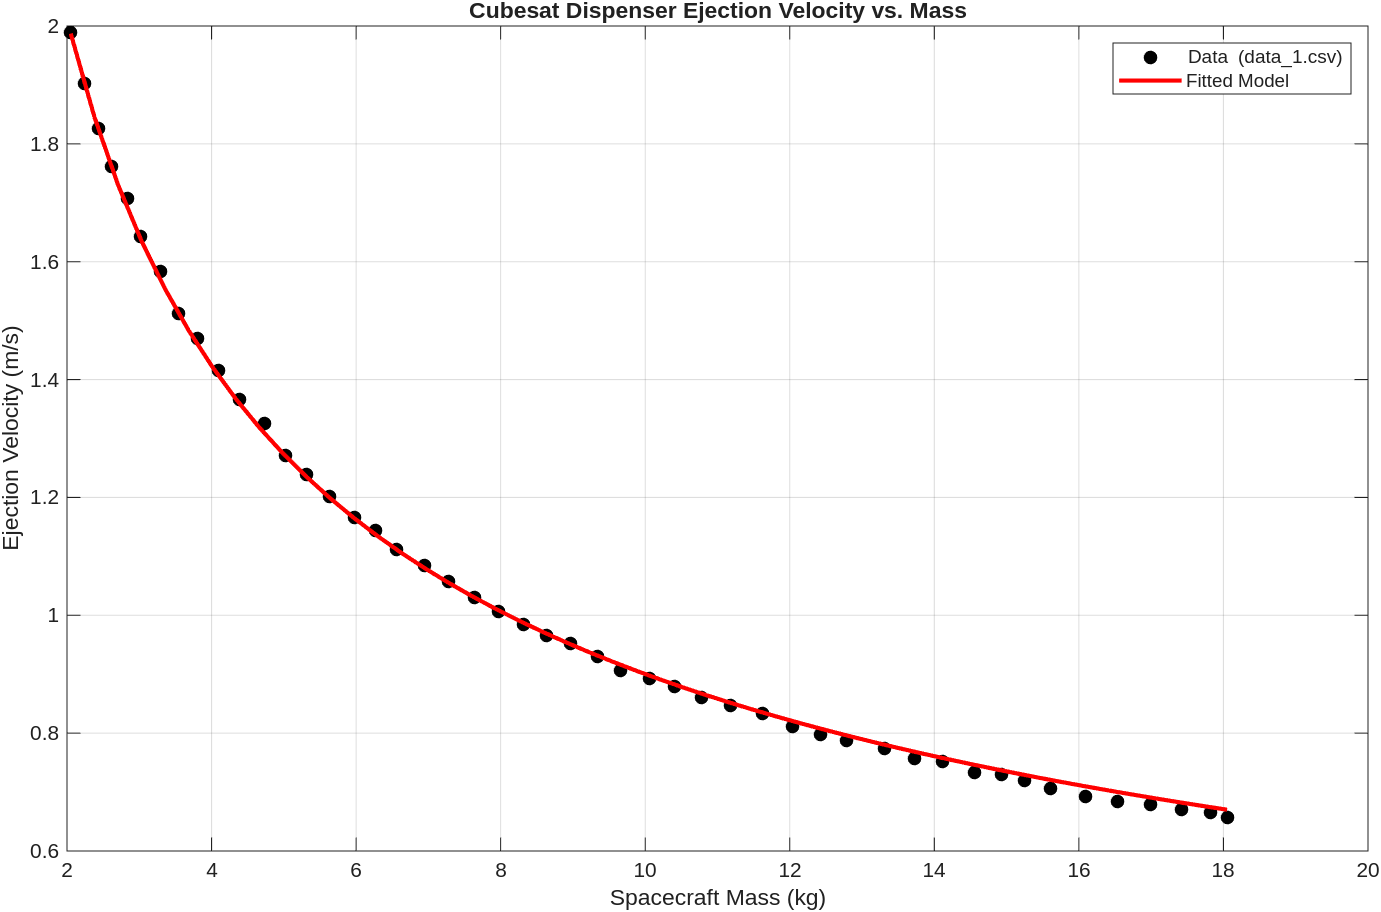
\includegraphics[keepaspectratio]{images/GNC_img_4.png}}

\end{minipage}%

\caption{\label{fig-mass-vel}Mass vs Veclocity: Simulated Curve and
Given data}

\end{figure}%

The MATLAB output is given below:

\begin{Shaded}
\begin{Highlighting}[]
\NormalTok{Generation 46/50 | Best Cost = 0.003424 | k = 360.2204 | b = 0.0000}
\NormalTok{Generation 47/50 started...}
\NormalTok{Generation 47/50 | Best Cost = 0.003424 | k = 360.2204 | b = 0.0000}
\NormalTok{Generation 48/50 started...}
\NormalTok{Generation 48/50 | Best Cost = 0.003424 | k = 360.2204 | b = 0.0000}
\NormalTok{Generation 49/50 started...}
\NormalTok{Generation 49/50 | Best Cost = 0.003424 | k = 360.2204 | b = 0.0000}
\NormalTok{Generation 50/50 started...}
\NormalTok{Generation 50/50 | Best Cost = 0.003424 | k = 360.2204 | b = 0.0000}

\NormalTok{ DE Optimization Complete}
\NormalTok{Best Cost                    : 0.0034241292}
\NormalTok{Estimated Spring Constant k  : 360.220434 N/m}
\NormalTok{Estimated Damping Coefficient b : 0.000020 Ns/m}
\end{Highlighting}
\end{Shaded}

From the above results, it can be seen that the estimated damping
coefficent is almost zero, \(b = 0.000020\ \mathrm{Ns/m}\). This shows
that the damping effect in the system is very small and can be
neglected. Hence, the system mainly behaves like a spring-mass system,
with the estimated spring constant of \(k = 360.220434\ \mathrm{N/m}\).
The simulated results obtained from these parameters are compared with
the given data in Figure~\ref{fig-mass-vel}.

\begin{quote}
Note: The optimized vriables and coast may differ at the runtime as it
depends on the \emph{rand} function, but \(k\) will remain close to
\(360.0\) and the \(b\) will remain close to \(0\).
\end{quote}

The objective function can be even reduced by running it for more
generation or the adding the tolerenace limit on the objective function.
The author belives that, it will lead to the cost function to zero and
the \(k = 360 \; and \; b = 0.0\).

\begin{figure}[H]

\begin{minipage}[t]{\linewidth}

\pandocbounded{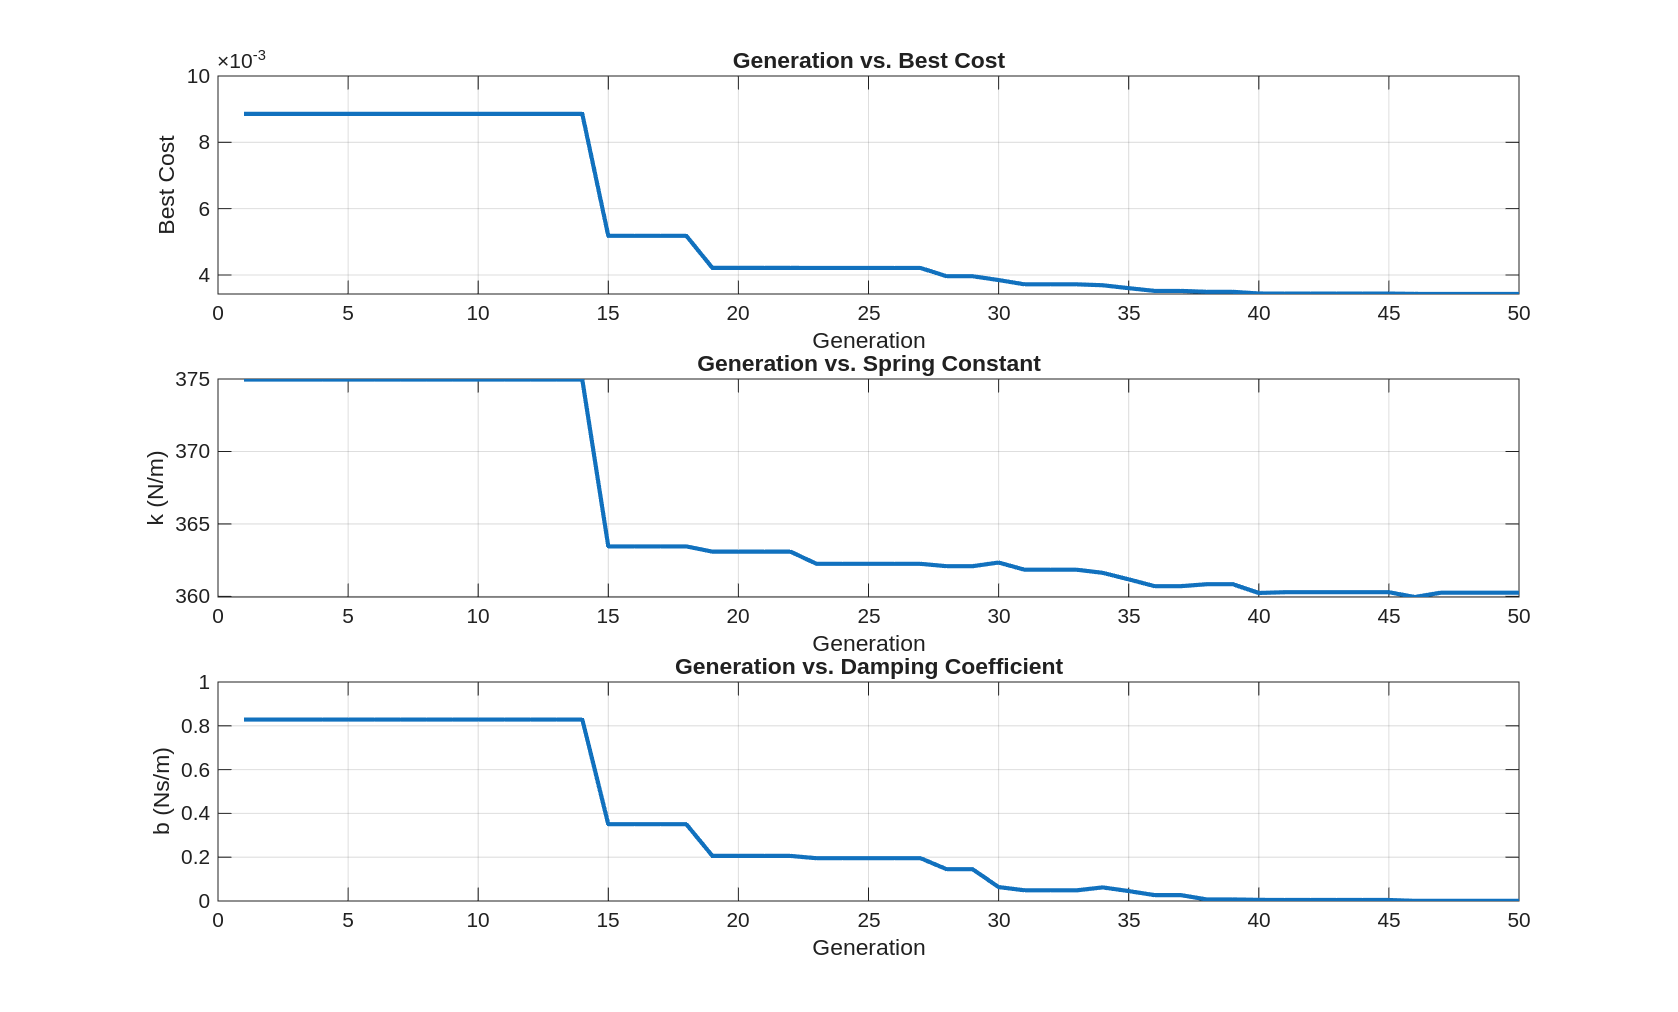
\includegraphics[keepaspectratio]{images/GNC_img_5.png}}

\end{minipage}%

\caption{\label{fig-obj-kb}Generation vs Coast, k and b}

\end{figure}%

\pagebreak


\renewcommand\refname{References}
\bibliography{references.bib}



\end{document}
